\documentclass[a4paper,11pt]{report}
\usepackage[T1]{fontenc}
\usepackage[utf8]{inputenc}
\usepackage{lmodern}
\usepackage{graphicx}
\usepackage{listings}
\usepackage[margin=1in]{geometry}
\usepackage[hidelinks]{hyperref}

\title{Command Line Control of an Asterisk Confbridge}
\author{Darryn Anton Jordan \\\href{mailto:jrddar001@myuct.ac.za}{jrddar001@myuct.ac.za}}

\begin{document}

\maketitle
\tableofcontents

\lstdefinestyle{customc}{
  belowcaptionskip=1\baselineskip,
  breaklines=true,
  frame=L,
  xleftmargin=\parindent,
  language=C++,
  showstringspaces=false,
  basicstyle=\footnotesize\ttfamily,
}

\newpage

\section{Introduction}
This document details the method used to configure an Asterisk server and describes a C++ program used to record calls made in a ConfBridge using the Asterisk Manager Interface (AMI).\\ The aim is to create a platform where node operators can group call through an Asterisk ConfBridge. 

\subsection{Software and Hardware Used}
\begin{itemize}
  \item Ubuntu 15.04
  \item Asterisk 13.1.0
  \item Code::Blocks 13.12
  \item Boost Asio Library
  \item SFLphone 1.4.1
\end{itemize}

\newpage

\section{Preparation and Set-up}
\subsection{Overview of system}
Each node is assigned a SIP account and an extension number. This number can be used for one-on-one calls. Furthermore, a ConfBridge is created. This is essentially a conference call with a specific extension. Recording of the ConfBridge is achieved using the developed C++ program. 
\subsection{Asterisk Server}
The server is required to have Asterisk installed:
\begin{lstlisting}
  sudo apt-get install asterisk
\end{lstlisting}
Once installed, the command line interface can be accessed as follows:
\begin{lstlisting}
  sudo asterisk -r
\end{lstlisting}
\begin{figure}[h]
  \begin{center}
    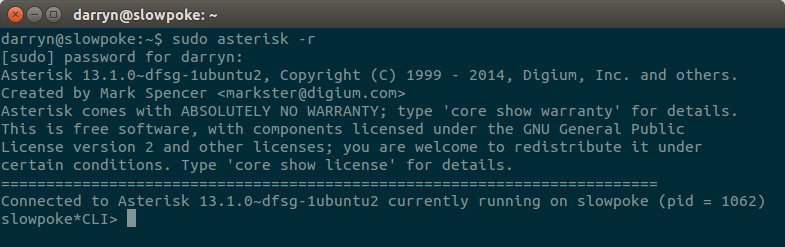
\includegraphics[scale = 0.4]{asterisk_cli}
    \caption{Asterisk CLI}
  \end{center}
\end{figure}
The Asterisk server is configured by editing four \textit{.conf} files: 
\begin{itemize}
   \item sip.conf - manage SIP accounts and set the server IP.
   \item extensions.conf - control what happens when extensions are dialled.
   \item confbridge.conf - configure a confbridge.
   \item manager.conf - allows control through the AMI.
 \end{itemize} 
These files are located at:
\begin{lstlisting}
  /etc/asterisk
\end{lstlisting}
These files must be replaced with the provided ones, in order to allow recording. It is recommended to make a copy of the original contents before replacing.

\subsection{Important CLI Commands}
\begin{itemize}
  \item Whenever a \textit{.conf} file is altered, the \textit{reload} command must be used to refresh the server.
  \item To restart the server, use \textit{core restart now}.
  \item View users present in a confbridge, \textit{confbridge list}. 
  \item Commands can be made from terminal, without entering the CLI:
\begin{lstlisting}
  sudo asterisk -rx "command"
  
For example:
  sudo asterisk -rx "confbridge list"
\end{lstlisting} 
\end{itemize}

\subsection{Configuration File Descriptions}

\subsubsection{sip.conf}
\lstset{escapechar=@,style=customc}
\lstinputlisting[style=customc]{sip.conf}

\subsubsection{extensions.conf}
\lstinputlisting[style=customc]{extensions.conf}

\subsubsection{manager.conf}
\lstinputlisting[style=customc]{manager.conf}

\subsubsection{confbridge.conf}
\lstinputlisting[style=customc]{confbridge.conf}

\newpage
\subsection{SIP Clients}
\subsubsection{SFLphone 1.4.1}
This client was used during testing of the asterisk server. Note that the status must be registered in order to work.
\begin{figure}[h]
  \begin{center}
    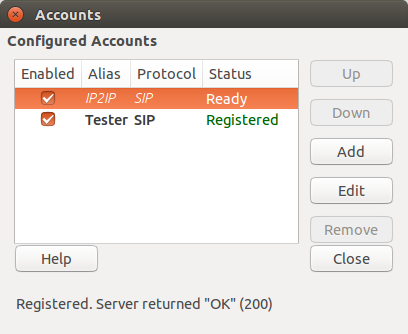
\includegraphics[scale = 0.4]{SIP_accounts}
    \caption{Account Settings}
  \end{center}
\end{figure} \\
Figures 3 and 4 display the account settings of a functioning account.
\begin{figure}[h]
  \begin{center}
    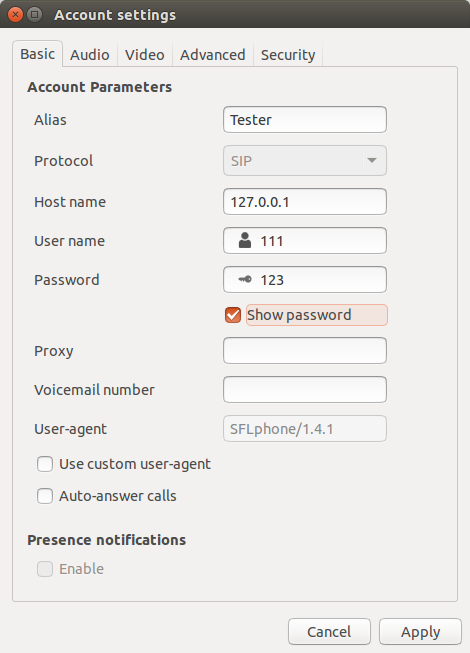
\includegraphics[scale = 0.4]{SIP_basic_settings}
    \caption{Basic Account Settings}
  \end{center}
\end{figure}

\newpage
\textbf{NB} Note that the port number is different to the one specified in the \textit{sip.conf} file.
\begin{figure}[h]
  \begin{center}
    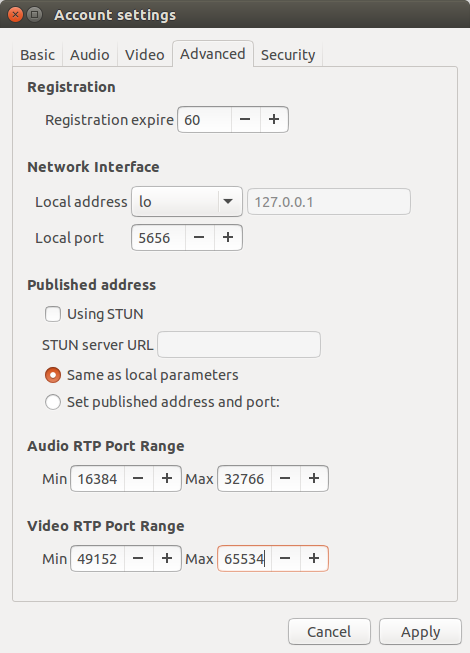
\includegraphics[scale = 0.4]{SIP_adv_settings}
    \caption{Advanced Account Settings}
  \end{center}
\end{figure}\\
To test the server confbridge, dial 100 using SFLphone. The user is prompted to speak his/her name and then press the hash key. The user is announced to any other users present in the confbridge  and the conference call commences.
\subsubsection{Linphone 3.6.1}
Linphone is a cross-platform SIP client (iOS, Android, Windows, OS X and Linux). It has been tested to work perfectly with this system on iOS and Linux. The set-up is extremely similar to the method described above. Friendly reminder: port number is 5656. (NOT 5060)

\section{C++ Confbridge Recorder}
Upon compiling the code in Code::Blocks, the following console application will appear:
\begin{figure}[h]
  \begin{center}
    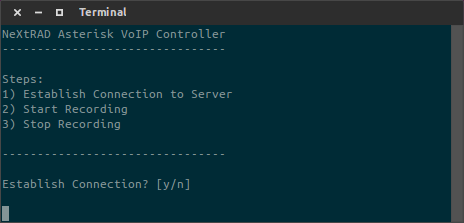
\includegraphics[scale = 0.5]{welcome}
    \caption{Welcome Screen}
  \end{center}
\end{figure}

\newpage 

The user is then breifly shown the background commands, afterwhich a prompt to start recording appears. If the program is successful in initiating recording, the output shown in Figure 6 will appear. 
\begin{figure}[h]
  \begin{center}
    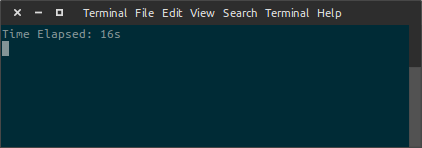
\includegraphics[scale = 0.5]{stop}
    \caption{Recording Success}
  \end{center}
\end{figure}\\
During development, the only location which Asterisk had permission to store recorded files was: /var/spool/asterisk \\
It is possible to store the recordings in any folder, if the folder is given full permissions using terminal: \textit{chmod 777 /path/to/folder}\\\\
\textbf{NB} Note that a confbridge only exists once a user is present. Thus, a user must be in the confbridge before recording can take place. The following error occurs if no users are present:
\begin{figure}[h]
  \begin{center}
    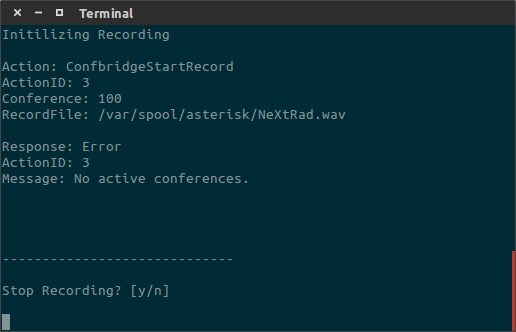
\includegraphics[scale = 0.5]{confbridge_error}
    \caption{Confbridge Error}
  \end{center}
\end{figure}\\

\newpage
\section*{Appendix A: Code Listing}

\lstset{escapechar=@,style=customc}
\lstinputlisting[style=customc]{main.cpp}



\end{document}
